% Chapter Template

\chapter{Discussion}

\label{sec:discussion} % Change X to a consecutive number; for referencing this chapter elsewhere, use \ref{ChapterX}

\lhead{\emph{Discussion}} % Change X to a consecutive number; this is for the header on each page - perhaps a shortened title

%----------------------------------------------------------------------------------------
%	SECTION 1
%----------------------------------------------------------------------------------------

\subsection{Towards an analytical description}
There is a key result of our simulations that allows us to build an
analytical description for the outgoing spectra.
It is the independence of the following three quantities with the rotational
velocity and the viewing angle: integrated flux, average number of
scatterings and escape fraction.
As we explained in \S~\ref{sec:intlineint}, the best way to understand this is that radiative transfer inside a sphere that undergoes solid-body rotation
proceeds identical to that inside a non-rotating sphere. While scattering events off atoms within the rotating cloud impart
Doppler boosts on the Ly$\alpha$ photon, these Doppler boost are only
there in the lab-frame. Therefore, in the frame of the rotating gas cloud all atoms are
stationary with respect to each other and the scattering process
proceeds identical as in the static case (also see \S~\ref{sec:intlineint} for an additional more quantitative explanation).
This result allows us to analytically estimate the spectrum emerging from a rotating cloud:
The spectrum of \lya photons emerging from a rotating gas cloud is identical as for the static case in a frame that is co-rotating
with the cloud. However, the surface of cloud now moves in the lab-frame.
Each surface-element on the rotating cloud now has a bulk
velocity with respect to a distant observer. In order to compute the
spectrum one can integrate over all the surface elements in the
sphere with their corresponding shift in velocity and an additional
weight by the surface intensity.
Fig~\ref{fig:comparison} shows some examples of analytic versus full MC
spectra using this approach (the implementation details are in the Appendix).
The left panel shows the results for different rotational velocities
in the case of $\tau_{H}=10^7$ and an observer located perpendicular
to the axis of rotation ($i=0$ in the scheme of Fig~\ref{fig:scheme}
in the Appendix). The right panel shows the results for different viewing angles in the
case of $\tau_{H}=10^7$ and a rotational velocity of $V_{\rm
max}=300$\kms.
The two methods clearly give good agreement, though not perfect. In particular, the left panel shows that the MC gives rise to a spectrum that is
slightly more concentrated towards the line centre. As we explain in Appendix~\ref{sec:app}, we do not expect perfect agreement, because this requires an analytic solution for the spectrum of Ly$\alpha$ photons emerging from a static, optically extremely thick cloud {\it as a function of the angle at which they escape from the sphere}. This solution does not exist in the literature. It is possible to get better agreement my modifying the surface brightness profile.
In any case, the analytic calculation closely captures the results
obtained from the full calculations from the MC simulations.
As such, they are extremely useful and provide us with a quick tool to
verify our calculations at the first order level.
\begin{figure*}
\begin{center}
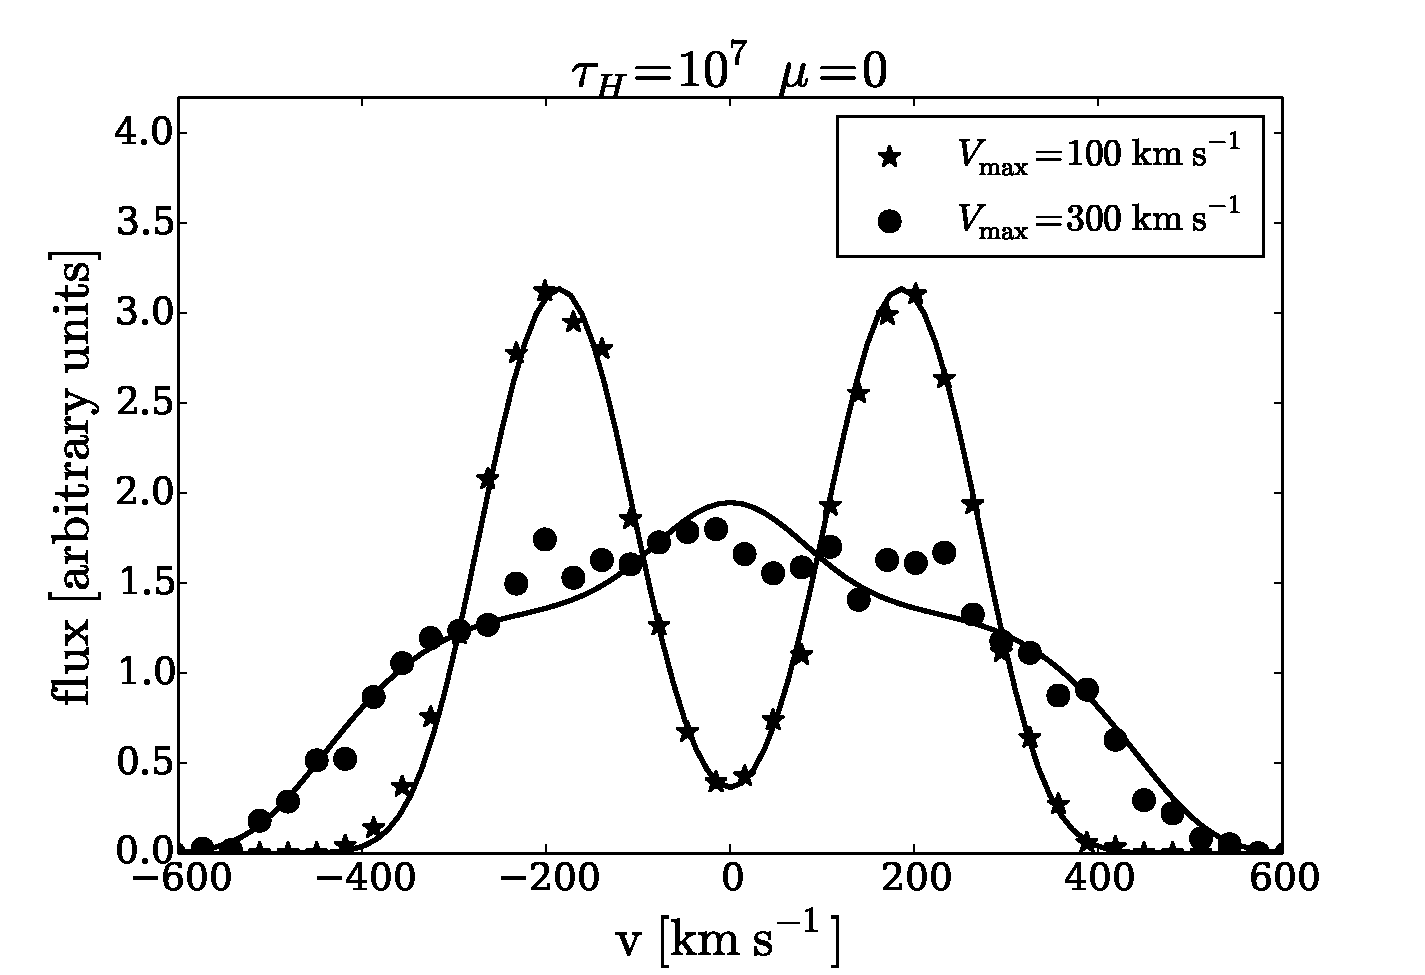
\includegraphics[width=0.49\textwidth]{../Figures/fig10a.pdf}
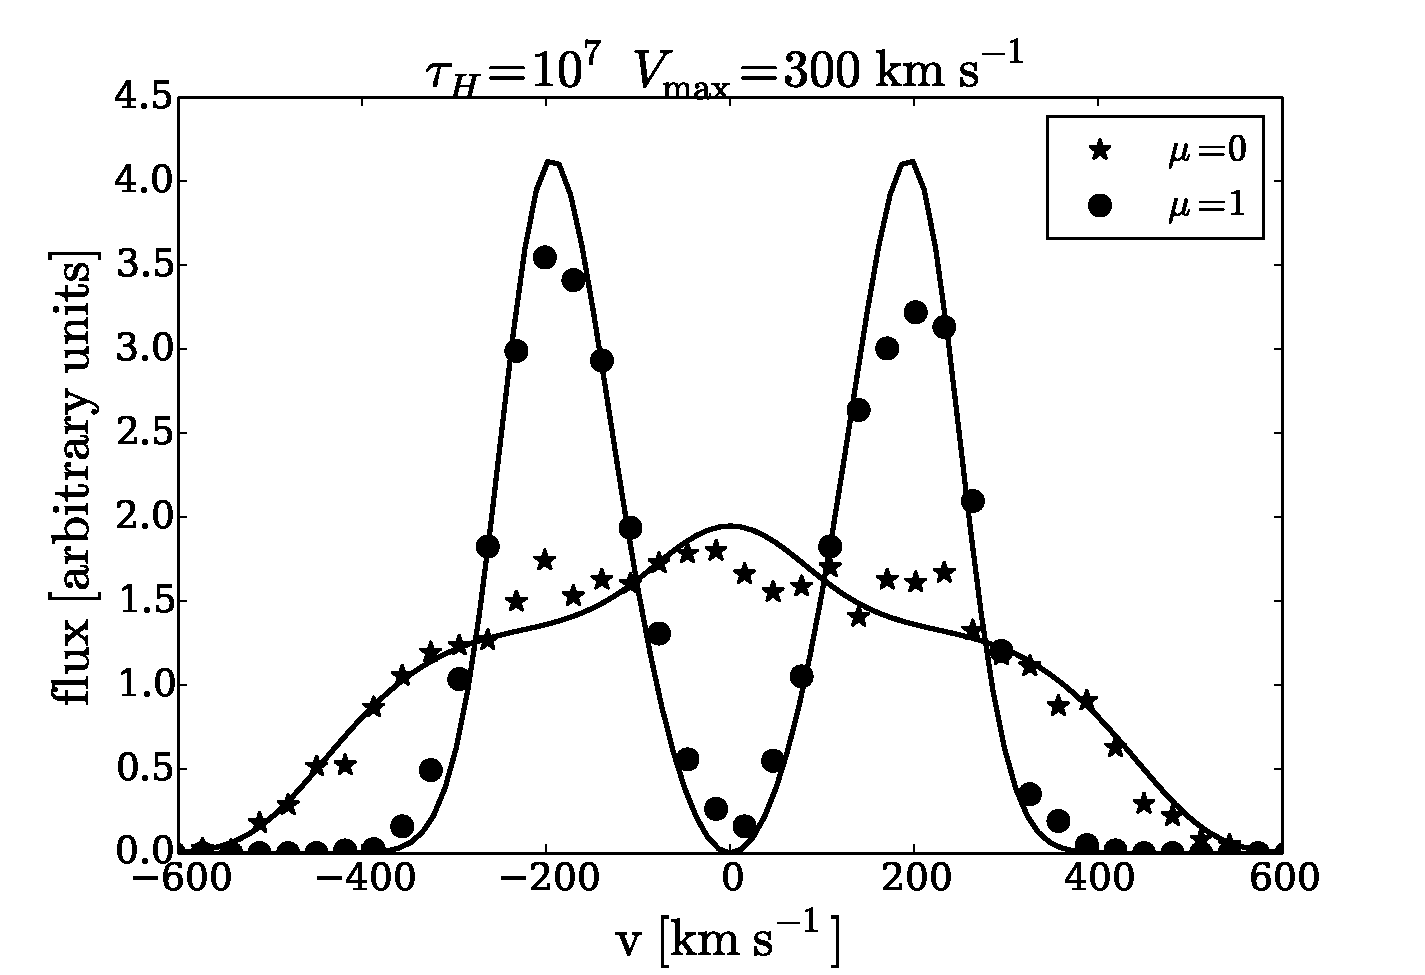
\includegraphics[width=0.49\textwidth]{../Figures/fig10b.pdf}
\end{center}
\caption{
Comparison of the Monte Carlo results against the analytic
solution. The left panel explores the results of different velocities.
The right panel presents the results for two different observers:
paralel and perpendicular to the rotational axis, $\mu=1$ and $\mu=0$
respectively.
\label{fig:comparison} }
\end{figure*}
\subsection{Impact on the interpretation of simulated and
observational data}
We now compare our findings to other computational results and discuss
its possible implications for the interpretation of observational data.
{\bf Escape at Line Center.} Our models have shown that rotation
enhances the flux density at line center (see Fig. \ref{fig:differentvelocities}). It has
recently been proposed that galaxies with Lya spectral lines that
contain flux at line center may be `leaking' ionizing (LyC) photons
\citep{Behrens2014,2014arXiv1404.2958V}. The main reason for this possible
connection is that the escape of ionizing (LyC) photons requires
$N_{\rm HI} < 10^{17} $cm$^{-2}$. The same low column densities facilitate the escape of
\ly photons at (or close to) line center. Our work suggests that
rotation may provide an alternative explanation.
{\bf Single peaked lines}. The presence of single peaked profiles has
been associated to inflow/outflow dynamics
\citep{Verhamme06,DijkstraKramer}.
Gas bulk rotation can also be considered as a probable origin for that
behaviour, provided that the observed single peak is highly
symmetric.
Similarly, in the case of double peaked lines with a high
level of flux at the line center, rotation also deserves to be
considered in the pool of possible bulk flows responsible for that feature,
specially if the two peaks have similar intensities.
{\bf Systemic velocities}. There are observational measurements for the
velocity shift between the \ly and other emission lines. In our study
we find that the position of the peak maxima can suddenly change with
rotation and viewing angle. Namely the line can become single peaked
for high rotational velocities and viewing angles perpendicular to the
rotation axis.
{\bf Galaxy simulations with gas rotation}. \cite{Verhamme12} studied \ly
line emission in two high resolution simulations of individual
galaxies.
The main purpose of their study was to assess the impact of two
different ISM prescriptions.
However, each simulated galaxy had a disc structure with a clear rotation pattern in
the ISM and inflowing gas from the circum-galactic region.
The configuration had an axial symmetry and they reported a strong dependence of both
the escape fraction and the total line intensity as a function of the
$\theta$ angle.
From our study, none of these two quantities has a dependence either
on the inclination angle or the rotational velocity.
We suggest that he effect reported by \cite{Verhamme12} is
consistent with being a consequence of the different hydrogen optical
depth for different viewing angles and not as an effect of the bulk
rotation.
{\bf Zero impact on the \ly escape fraction}. Study of
high redshift LAEs in numerical simulation often requires the
estimation of the \ly escape fraction in order to compare their
results against observations
\citep{CLARA,Dayal2012,Forero12,Orsi12,Garel2012}. Most of these
models estimate the escape fraction from the column density of dust and
neutral Hydrogen. The results of our simulation indicate that the
rotational velocity does not induce additional uncertainties in those
estimates.

